% Generated by code/scripts/report_figures.py at 2026-11-03T07:57:50Z; do not edit.
% Inputs: artifacts/local/runs/pipeline-e2e-20261103T075711Z/run
\begin{figure}[t]
\centering
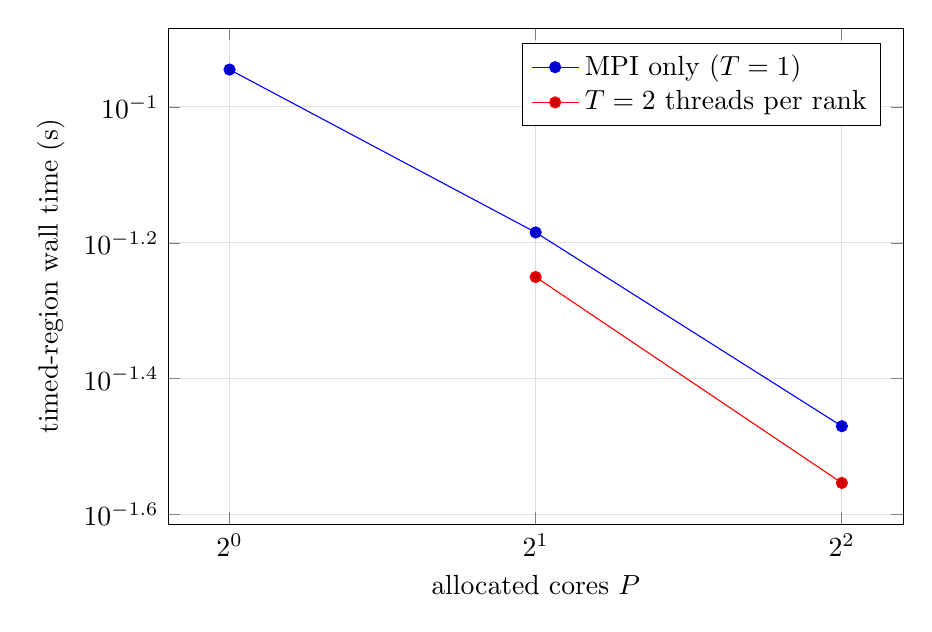
\begin{tikzpicture}
\begin{axis}[width=0.9\columnwidth, height=0.65\columnwidth, xlabel={allocated cores $P$}, ylabel={timed-region wall time (s)}, xmode=log, log basis x=2, ymode=log, legend pos=north east, legend cell align=left, grid=major, grid style={gray!25}]
\addplot+[mark=*] coordinates {(1,0.1135) (2,0.06537) (4,0.0339)};
\addlegendentry{MPI only ($T=1$)}
\addplot+[mark=*] coordinates {(2,0.0562) (4,0.02797)};
\addlegendentry{$T=2$ threads per rank}
\end{axis}
\end{tikzpicture}
\caption{\textbf{LOCAL PIPELINE TEST, NOT A MEASUREMENT.} Strong-scaling runtime. $N=4000$, median of repetitions; serial Barnes--Hut baseline on the same CPU model and build.}
\label{fig:strong-runtime}
\end{figure}
